\documentclass[a4paper,12pt]{article}

\usepackage[utf8]{inputenc}
%\usepackage{lipsum}
\usepackage{amsmath,amsthm,mathrsfs}
\usepackage[english]{babel}
\usepackage{textcomp}
%\usepackage[T1]{fontenc}
\usepackage{graphicx,wrapfig}
\usepackage{amssymb}

\newcommand\norm[1]{\left\lVert#1\right\rVert}
\usepackage{calc}
\usepackage{rotating}
\usepackage[usenames,dvipsnames]{color}
\usepackage{fancyhdr}
%\usepackage{subfigure}
\usepackage{hyperref}
\usepackage{longtable}
\usepackage{svg}
\usepackage{float}
\usepackage{rotating}
\usepackage[usenames,dvipsnames]{color}
\usepackage{fancyhdr}
%\usepackage{subfigure} 
\usepackage{hyperref}

\usepackage[utf8]{inputenc}
\usepackage[english]{babel}
\usepackage[backend=bibtex,
style=numeric,
bibencoding=ascii,
sorting=none
%style=alphabetic
%style=reading
]{biblatex}
\addbibresource{mid_sem2}
\usepackage[a4paper, margin=1.5in]{geometry}
\usepackage{pifont}
\usepackage{xcolor}
\usepackage{dirtytalk}
\hypersetup{
    colorlinks,
    linkcolor={red!50!black},
    citecolor={blue!50!black},
    urlcolor={blue!80!black}
}
\graphicspath{{images/}}
%\usepackage{times}
%\usepackage[scaled=0.8]{beramono}
 \renewcommand{\familydefault}{\rmdefault}

\begin{document}

\begin{titlepage}
\pagenumbering{gobble}
\begin{center}

 
%	\noindent\rule[0.5ex]{\linewidth}{4pt}
%  

  \vskip.1in
  \textbf{\Large Robust Controller Design Using \textbf{$H_{\infty}$}-Loop Shaping Approach}  \vskip.7in
  \vskip.7in
%\noindent\rule[0.5ex]{\linewidth}{4pt}
	\begin{center}\textit{\small{Mid-sem evaluation report submitted in partial fulfillment to the requirements}} \\
	\textit{\small{for the degree of}}
	\vskip.5in
	\large{\normalsize BACHELOR OF TECHNOLOGY}
	\vskip.3in
	\textit{by}
	\vskip.3in
	
	\textbf{\normalsize AYUSH PANDEY}\\
	\end{center}
\end{center}
%\vskip1.3in
%\begin{minipage}[t]{7cm}
%\flushleft
%\textsc{Author:}
%%
%Ayush Pandey \\12IE32001\\ IIT Kharagpur \\
%\end{minipage}
%\hfill
%\begin{minipage}[t]{7cm}
%\flushright
%\textsc{Supervisor:}
%
%Dr. Sourav Patra \\IIT Kharagpur
%\end{minipage}
%\vskip1.2in
\vskip.9in
\vskip.9in
\vskip.3in

\begin{center}

\includegraphics[scale=0.18]{logo}
\vskip.1in
\textbf{Department of Electrical Engineering}
\\
Indian Institute of Technology, Kharagpur
\\
West Bengal, INDIA 721302\\
November 2015

\end{center}
\end{titlepage}

\begin{wrapfigure}[1]{l}{0.001\textwidth}

\includegraphics[width=0.15\textwidth]{logo}
\end{wrapfigure}

\setlength{\parindent}{85pt}

 \large{Department of Electrical Engineering\\
} \-\hspace{3cm}\normalsize{Indian Institute of Technology, Kharagpur}
\\
 \-\hspace{3cm}West Bengal, INDIA 721302\\
 \-\hspace{3cm}November 2015\\ \\
\rule[2pt]{1.1\linewidth}{1pt}
\vskip.9in
\begin{center} \Large{\textbf{Certificate}} \end{center}
\vskip.4in
{\setlength{\parindent}{0cm}This is to certify that the report entitled \textbf{Robust Controller Design Using
$H_{\infty}$ Loop Shaping Approach}, submitted by \textbf{Ayush Pandey}, an undergraduate student, in the \textit{Department of Electrical Engineering, Indian Institute of Technology,
Kharagpur, India,} for the award of the degree of Bachelor of Technology, is a record of
the work carried out by him under our supervision and guidance. Neither this report nor any part of it has been submitted for any degree or academic award elsewhere.}
\vskip.9in
\vskip.9in
\parindent=0em
\begin{minipage}[p]{10cm}
\begin{flushleft}
\textbf{Dr. Sourav Patra}
\\Assistant Professor,\\
Department of Electrical Engineering,\\ Indian Institute of Technology,
Kharagpur,\\ INDIA 721302
\end{flushleft}
\end{minipage}

\vskip.9in
\vskip.9in
\vskip.9in
\vskip.9in
{\hypersetup{linkcolor=blue}
\tableofcontents
}
\vskip.9in
\vskip.9in
\vskip.9in
\vskip.9in
\vskip.9in
\vskip.9in
\section{Introduction}
%write in short the aim of the project and write about what has been done and what is the aim now.
This project deals with the analysis and design of a $H_{\infty}$ loop shaping controller using convex optimization based methods.
A brief introduction to the project was given in \cite{prev}. This document reports the subsequest work done. The reader is referred to \cite{prev} for detailed results and discussions on preliminaries to robust control theory, $H_{\infty}$ control, linear fractional transformation, small gain theorem for robust stability analysis and a few examples on these topics. \\
The $H_{\infty}$ loop shaping design technique incorporates classical loop shaping method to obtain performance and robust stability tradeoffs along with $H_{\infty}$ control optimization technique to gurantee a level of closed loop robust stability. This method ensures robustness against unstructured uncertainty which is described as perturbations to normalized coprime factors of the shaped plant. \\
The first two sections of this report give a brief discussion of solution of $H_{\infty}$ control problem by finding out the $H_{\infty}$ norm using a convex optimization technique. The preliminaries for the same have been covered and related proofs have been presented. The second section ends with a few examples on the same. The next section covers coprime factor uncertanity description to a plant, its robust stabilization and $H_{\infty}$ loop shaping design procedure. The report ends with a justification on how this technique leads to a good and acceptable robust controller design.
\section{Preliminaries}
Various robust control theory preliminaries such as matrix norms, performance specifications, $H_{\infty}$ and $H_{2}$ norms, coprime factorization, linear fractional transformation etc. have been covered in \cite{prev}. This section gives an introduction to  convex optimization based technique to solve the $H_{\infty}$ control optimization problem. Before 1995, two algebraic riccati equation based methods were used to solve the $H_{\infty}$ control optimization problem, the disadvantage with these methods is that they require various assumptions to be satisfied which are usually not satisfied for many plant models. A convex optimization based approach was proposed in the mid 90s which was based on solving a few linear matrix inequalities (LMIs) inorder to result in a stabilizing controller for the $H_{\infty}$ control problem. The LMI based approach is easily applicable to a range of systems and is covered in detail in Section \ref{h}.
	\subsection{Linear Matrix Inequality}
	An optimization problem with convex constraints can be formulated in the LMI framework. An LMI has the following form.
		\begin{equation}
			\label{lmi_eq}
			F(x)=F_{0}+\sum_{i=1}^{m}x_{i}F_{i} > 0
		\end{equation}
		where, $x=[x_{1} x_{2} ... x_{m}]$ is the design variable and $F_{i}$, $i=0,1...m$ are symmetric matrices. The constraint shown in Eq.(\ref{lmi_eq}) indicates the positive definiteness of the matrix $F(x)$. Formulation of an optimization problem in the LMI framework helps the designer to make use of the available LMI solvers in softwares such as MATLAB to efficiently solve the optimization problem.
	\subsection{Bounded Real Lemma}
	As previously seen in \cite{prev}, closed loop performance and robust stability requirements for a system expressed in LFT framework can be expressed as $H_{\infty}$ norm minimization problem of certain stable closed loop transfer function matrix of the form $\norm{T_{zw}}_{\infty} < \gamma$. 
	The bounded real lemma gives equivalent conditions to this minimization in LMI framework which can be solved to effectively solve the $H_{\infty}$ control problem. Consider a system in state space representation as follows.
	\begin{align}
	\label{ss}
		\textbf{\.x}&=\textbf{Ax} + \textbf{Bu}, x(0)=0\\
		\textbf{y}&=\textbf{Cx} + \textbf{Du}
		\end{align}
		In compact matrix notation, we can write (denoting the system TFM as G(s)):
		\[G(s)=\begin{bmatrix}
		\begin{array}{c|c}
		A & B \\\hline C & D
		\end{array}
		\end{bmatrix}
		\]
		The bounded real lemma states that 
		$\norm{G(s)}_{\infty}<\gamma \Leftrightarrow \exists \: Y = Y^{T} > 0$ such that:
		\begin{align}
		\label{brl_lmi}
		\begin{bmatrix}
		YA+A^{T}Y & YB & C^{T} \\
		B^{T}Y & -\gamma I & D^{T}\\
		C & D & -\gamma I
		\end{bmatrix}
		< 0
		\end{align}
		The above LMI can be solved for $Y$ and $\gamma$ using convex optimization techniques. The value of $\gamma$ corresponds to the $H_{\infty}$ norm of the TFM $G(s)$ which can be used to design a stabilizing controller. 
		\paragraph{Proof} We can write 
		\begin{align}
		\norm{G(s)}_{\infty} = \sup_{u\neq0} \frac{\norm{y}_{2}^{2}}{\norm{u}_{2}^{2}}
		\label{hn2}
		\end{align} 
		We have, $\norm{G(s)}_{\infty}<\gamma$ and we need to derive the relation in Eq.(\ref{brl_lmi}). We define a supply rate function as $(\gamma^{2}\norm{u}_{2}^{2} - \norm{y}_{2}^{2})$. From Eq.(\ref{hn2}), we have that the supply rate function is positive. Physically, this is the energy supply rate to a system whose input is $u$ and output, $y$. Let, $V(x)$ be the energy storage function for this system. Then, we directly have that
		\begin{equation}
			\dot{V}(x) < (\gamma^{2}\norm{u}_{2}^{2} - \norm{y}_{2}^{2})
			\label{one} 
		\end{equation}		 
		That is, the rate of supply of energy to the system would always be more than the rate of storage of energy in the system. For a linear time invariant systems with minimal realization, this function $V(x)$ can be considered to be the Lyapunov function of the system. Now, let $V(x)$ be a quadratic Lyapunov function $x^{T}Px$. For the system in Eq.(\ref{ss}), we evaluate Eq.(\ref{one}) and on simple manipulation we get,\\
		
		\[
		\Leftrightarrow
		\begin{bmatrix}
		x^{T} & u^{T}
		\end{bmatrix}
		\begin{bmatrix}
		A^{T}P+PA+C^{T}C & PB+C^{T}D \\
		B^{T}P+D^{T}{C} & -\gamma^{2} I + D^{T}D
		\end{bmatrix}
		\begin{bmatrix}
		x \\ u
		\end{bmatrix}
		<0
		\]
		\\
		
		\[
		\Leftrightarrow
		\begin{bmatrix}
		A^{T}P+PA+C^{T}C & PB+C^{T}D \\
		B^{T}P+D^{T}{C} & -\gamma^{2} I + D^{T}D
		\end{bmatrix}
		< 0
		\]
		Now, we know that for a function to be a Lyapunov function candidate, the following properties are satisfied:
		\begin{enumerate}
		\label{ly}
		\item $V(0)=0$ 
		\item $V(x)>0\: \forall\: x\:\neq\:0$
		\end{enumerate}Using this and the fact that for an LTI system stability doesn't depend on the input, we can see from Eq.(\ref{one}) that the system is stable as $\dot{V}(x) < 0$. On integrating Eq.\ref{one} for time $0$ to time $t$, we obtain
		\begin{align}
		&\Leftrightarrow V(x(t))-V(x(0)) < \int\limits_{0}^{t} (\gamma^{2}\norm{{u}_{2}}^{2} - \norm{{y}_{2}}^{2}) dt\\
		\intertext{Since $x(0)=0$, We have $V(x(0))=0$ and $V(x(t))$ is always positive. Hence,}
		&(\gamma^{2}\norm{u}_{2}^{2} - \norm{y}_{2}^{2}) > 0\\
		&\Leftrightarrow\frac{\norm{y}_{2}^{2}}{\norm{u}_{2}^{2}} < \gamma^{2}\\
		&\Leftrightarrow\norm{G(s)}_{\infty} < \gamma
		\end{align}
		We have proved that $\norm{G(s)}_{\infty} < \gamma$ is equivalent to, when $\exists Y=Y^{T} > 0$ such that 
		\[		
		\begin{bmatrix}
		A^{T}P+PA+C^{T}C & PB+C^{T}D \\
		B^{T}P+D^{T}{C} & -\gamma^{2} I + D^{T}D
		\end{bmatrix}
		< 0
		\]
		Now, using the Schur's complement lemma, we will prove the statement of the bounded real lemma. The Schur's complement lemma for a symmetric matrix states that
		\[
		\begin{bmatrix}
		A & B \\ B^{T} & D
		\end{bmatrix}
		< 0
		\Leftrightarrow
		A-BD^{-1}B^{T} < 0\: ; \:D < 0
		\Leftrightarrow
		D-B^{T}A^{-1}B < 0 \: ; \: A < 0
		\]
		For the LMI in the bounded real lemma statement, using Schur's complement taking 
		\[
		A=
		\begin{bmatrix}
		YA+A^{T}Y & YB \\
		B^{T}Y & -\gamma I 
		\end{bmatrix}
		,\:B=
		\begin{bmatrix}
		 C^{T} \\
		D^{T}
		\end{bmatrix}
		,\:D=
		\begin{bmatrix}
		-\gamma I
		\end{bmatrix}
		\]
		Using the above matrices in the Schur's complement's first form, we can prove the equivalence relation in the bounded real lemma, which completes the proof. 
\section{LMI Based Approach to $H_{\infty}$ Control}
\label{h}
As mentioned in the Introduction section, there are three methods to solve a $H_{\infty}$ control problem. The first two methods, viz. the DGKF method and the Doyle-Glover method are based on finding out a stabilizing solution to certain algebraic riccati equation. The design procedure in these methods works only when the system satisfies a set of assumptions which are usually difficult to satisfy for a given plant model. On the other hand, the LMI based convex optimization approach only requires two assumptions mentioned in the next section, which are satisfied easily for a range of different systems. Also, it has been proved that  the controller structure found in the two methods can be similarly derived in the LMI framework. Hence, the LMI based approach to $H_{\infty}$ control is widely used due to its ease of design on the part of the designer.
	Using the bounded real lemma stated and proved in the previous section, the $H_{\infty}$ norm of a TFM can be found out by solving the LMI. This can be used to design a stabilizing controller $K(s)$ for a system by minimizing the $H_{\infty}$ norm of the closed loop TFM. The LMI approach to $H_{\infty}$ control requires two assumptions to be satisfied for the generalized plant $P$. Let a generalized plant be expressed in state space representation as follows.
	\[
	P=\begin{bmatrix}
	\begin{array}{c|cc}
	A & B_{1} & B_{2}\\ \hline
	C_{1} & D_{11} & D_{12} \\ 
	C_{2} & D_{21} & D_{22}	
	\end{array}
	\end{bmatrix}
	\]
	The following two assumptions should be satisfied to apply LMI based approach to solve the $H_{\infty}$ control problem:
	\begin{enumerate}
		\item ($A$,$B_{1}$,$C_{1}$) stabilizable and detectable.
		\item $D_{22} = 0$
	\end{enumerate}
	The controller design to minimize the $H_{\infty}$ norm of the generalized plant using LMI approach has been covered in detail in \cite{Pasca}. A simple numerical example is shown in the next section which demonstrates the use of LMI toolbox and YALMIP toolbox to calculate the $H_{\infty}$ norm of a given system in MATLAB using bounded real lemma. 
	\subsection{Examples and Simulations}
	In \cite{prev}, we took a simple stable system and calculated its infinity norm.
		\[A=\begin{bmatrix}
		-1 & 0 \\
		0 & -3
		\end{bmatrix}
		,\:B=\begin{bmatrix}
		0 & 1 \\
		2 & 1
		\end{bmatrix}
		,\:C=\begin{bmatrix}
		1 & 2 \\ 1 & 0
		\end{bmatrix}
		, D= 0_{2 \times 2}
		\]
		Using MATLAB's Robust Control Toolbox \textit{hinfnorm} function, the value obtained was 2.2836. The same result will be shown in the following sections obtained by solving the LMI that the bounded real lemma gives using the LMI tooblox and the YALMIP toolbox \cite{yalmip}. 
		\subsubsection{LMI Toolbox} The \textit{mincx} function in MATLAB helps in minimizing linear objective under LMI constraint. To use this, first an LMI needs to be defined using \textit{setlmis}, \textit{lmivar} and \textit{lmiterm} commands. The details for these commands are available in MATLAB documentation. After an LMI has been defined in MATLAB, the linear objective function which needs to be minimized is defined using \textit{defcx} function. Once this is done, the \textit{mincx} command yields the minimized objective function value as well as the value at which this minimum occurs. This completes the $H_{\infty}$ norm calculation. The MATLAB code written for the above system is avaliable at \cite{git}. 
		\subsubsection{YALMIP Toolbox}
		YALMIP is a modelling language for advanced modeling and solution of convex and nonconvex optimization problems. Its function \textit{optimize} can be used to solve a convex optimization problem. The YALMIP toolbox code works on symbolic decision variables which are defined by the user. These decision variables can be then used to define the LMI in a very user friendly manner. YALMIP toolbox can be used to solve both strict and non-strict constraint LMIs while MATLAB's LMI toolbox only handles strict constraints. For the system shown above, the MATLAB program which solves the LMI given by the bounded real lemma is available at \cite{git}. As expected, the result for the $H_{\infty}$ norm is same using all the three methods.
\section{$H_{\infty}$ Loop Shaping Control} The $H_{\infty}$ controller design optimization methods face a few disadvantages with respect to model perturbations being limited by number of poles in the RHP and the possibility of undesirable pole-zero cancellation between the nominal plant and the $H_{\infty}$ controller. In $H_{\infty}$ loop shaping design technique, the perturbations are directly described on the coprime factors of the nominal model. This helps in relaxing the restriction on the number of RHP poles and also doesn't produce any pole-zero cancellation. More importantly, this design technique is computationally more efficient as it doesn't require an iterative procedure for finding $\gamma$. Finally, since this design technique inherits concepts of loop shaping which is a classical controller design technique, hence it is much more user friendly method to design a robust controller.
	\subsection{Coprime Factor Uncertainty Description} A brief introduction to coprime factorization was given in \cite{prev}. We consider left coprime facotrization of a plant $P$ given by $\tilde{M}^{-1}\tilde{N}$, where $\tilde{M}$ and $\tilde{N} \in \mathbb{RH}_{\infty}$. 
%	\begin{figure}[H]
% 
%			  \centering
%			  
%			  \includesvg[width=1.0\textwidth]{block2}
%%			  \def\svgscale{5.5}
%%			  \tiny{
%%			  \input{ulft.pdf_tex}}
%			  \caption{Coprime Factor Uncertainty Description Block Diagram}
%			 \label{co1}
%		\end{figure}	
	Unstructured uncertainties can be described in a more general sense by perturbations on the coprime factors of a plant ($\tilde{\Delta}_{m}$ and $\tilde{\Delta}_{n} \in \mathbb{RH}_{\infty}$). The Figure(\ref{co2}) shows perturbations on the left coprime factors of the plant $P$ considered above. 
		\begin{figure}[H]
			  \centering
			  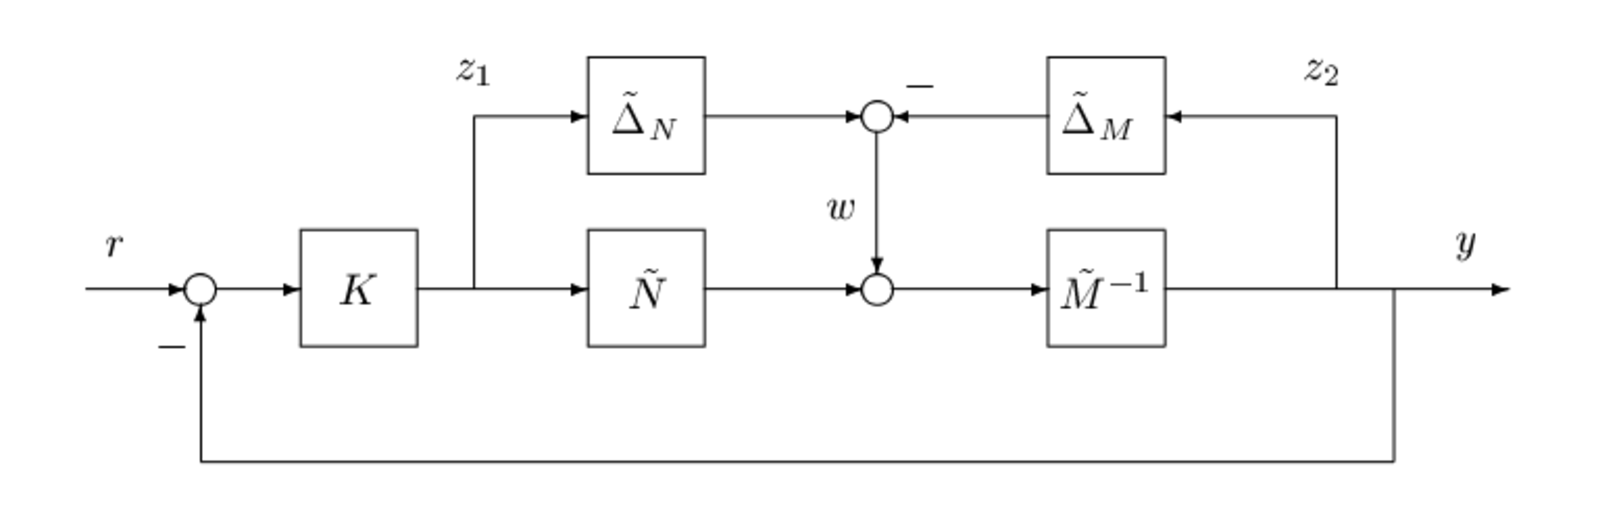
\includegraphics[scale=0.5]{co2}
%			  \includesvg[width=1.0\textwidth]{co}
%			  \def\svgscale{5.5}
%			  \tiny{
%			  \input{co2.pdf}}
			  \caption{Perturbations to Coprime Factors : Block Diagram}
			 \label{co2}
		\end{figure}	From the block diagram we have,
	
	\begin{align}
	y_{1}&=\tilde{M}y\\
	y_{1}&=\tilde{N}u + \tilde{\Delta}_{n}u - \tilde{\Delta}_{m}y\\
	\intertext{We have from these two equations, eliminating $y_{1}$} 
	y&=(\tilde{M} + \tilde{\Delta}_{m})^{-1}(\tilde{N}+\tilde{\Delta}_{n})u
	\end{align}
	Hence, the perturbed plant in this case is given by
	\begin{equation}
		\label{P}
		P =(\tilde{M} + \tilde{\Delta}_{m})^{-1}(\tilde{N}+\tilde{\Delta}_{n})
	 \end{equation}
	 Now with this coprime factor perturbed plant, we will study the robust stabilization and the $H_{\infty}$ loop shaping controller design technique.
	\subsection{Robust Stabilization of Coprime Factors} In Eq.(\ref{P}), we assume that $\norm{[\tilde{\Delta}_{m} \:\: \tilde{\Delta}_{n}]}_{\infty} < \epsilon$. We assume that in Fig.(\ref{co2}) the controller $K$ internally stabilizes the nominal plant. The robust stability analysis for this system can be done by reducing the block diagram in Fig.(\ref{co2}) to LFT framework and applying the small gain theorem. For the equivalent $M-\Delta$ structure, we can obtain $M$ as follows.
	
	%%%% WRITE STEPS%%%%
	
	
	\begin{align*}
	M=\begin{bmatrix}
	K \\ I
	\end{bmatrix}
	(I+PK)^{-1}\tilde{M}^{-1}
	\end{align*}	 
	
	Hence, on using small gain theorem, we obtain the following condition for robust stability of the system.
	\begin{equation}
	\norm{\begin{bmatrix}
	K \\ I
	\end{bmatrix}
	(I+PK)^{-1}\tilde{M}^{-1}}_{\infty} \leq \frac{1}{\epsilon}	
	\end{equation}
	
	Now, the following theorem from coprime factorization theory could be used to derive the generalized plant expression for the system shown in Fig.(\ref{co2}).
	The theorem gives the left and right coprime factorizations for a proper real-rational TFM. Let a system P have the following stabilizable and detectable state space realization.
	\[P =
	\begin{bmatrix}
	\begin{array}{c|c}
	A & B \\ \hline
	C & D	
	\end{array}
	\end{bmatrix}
	\]
	Now, let B and L be matrices such that $A+LC$ and $A+BF$ are both stable. Then we can define:
	\begin{equation}
	\begin{bmatrix}
	M & -Y_{l} \\
	N & X_{l}
	\end{bmatrix}
	=
	\begin{bmatrix}
	\begin{array}{c|cc}
	A+BF & B & -L \\ \hline
	F & I & 0\\ 
	C+DF & D & I
	\end{array}
	\end{bmatrix}
	\end{equation}
	\begin{equation}
	\begin{bmatrix}
	X_{r} & Y_{r} \\
	-\tilde{N} & \tilde{M}
	\end{bmatrix}
	=
	\begin{bmatrix}
	\begin{array}{c|cc}
	A+LC & -(B+LD) & L \\ \hline
	F & I & 0\\ 
	C & -D & I
	\end{array}
	\end{bmatrix}
	\label{mn}
	\end{equation}
	Then $P\:=\:NM^{-1}\:=\:\tilde{M}^{-1}\tilde{N}$ are rcf and lcf respectively. The above theorem can be proved by verifying the Bezout's identity for double coprime  facotrization of plant P. Now, using Eq.(\ref{mn}), we get the following result for lcf of $P$.
	\begin{equation}
	\begin{bmatrix}
	\tilde{N} & \tilde{M}
	\end{bmatrix}
	= \begin{bmatrix}
	\begin{array}{c|cc}
	A+LC & B+LD & L \\ \hline C & D & I	
	\end{array}
	\end{bmatrix}
	\label{mn2}
	\end{equation}
	Using Eq.(\ref{mn2}) and denoting the controller $\hat{K}=-K$ in Fig.(\ref{co2}), we have for $z=[z_{1}\: z_{2}]^{T}$
	\begin{align*}
	z_{1} &= u \\
	z_{2} &= \tilde{M}^{-1}w + \tilde{M}^{-1}\tilde{N}u\\
	y &= \tilde{M}^{-1}w + \tilde{M}^{-1}\tilde{N}u
	\end{align*}
	Hence, the generalized plant in the equivalent closed loop LFT structure (as shown in Fig.(\ref{lft})) is as follows (in the transfer function form).
	\begin{figure}[H]
			  \centering
			  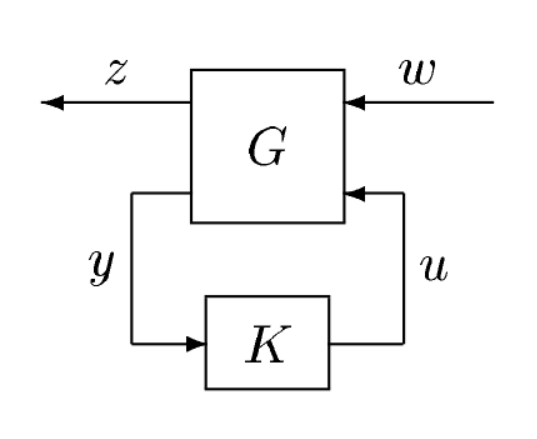
\includegraphics[scale=0.3]{lft}
%			  \includesvg[width=1.0\textwidth]{co}
%			  \def\svgscale{5.5}
%			  \tiny{
%			  \input{co2.pdf}}
			  \caption{Lower LFT Representation}
			 \label{lft}
		\end{figure}
	\begin{equation}
	G(s) = \begin{bmatrix}
	\begin{bmatrix}
	0\\\tilde{M}^{-1}
	\end{bmatrix} & \begin{bmatrix}
	I \\ P
	\end{bmatrix} \\
	\tilde{M}^{-1} & P
	\end{bmatrix}
	\end{equation}
	And in state space form is given by
	\begin{equation}
	G=\begin{bmatrix}
	\begin{array}{c|cc}
	A & -L & B\\ \hline
	\begin{bmatrix}
	0 \\ C
	\end{bmatrix}
	 & \begin{bmatrix}
	 0 \\I
	 \end{bmatrix}
	  & \begin{bmatrix}
	  I \\D
	  \end{bmatrix} \\
	  C & I & D
	\end{array}
	\end{bmatrix}
	\label{ssnm}
	\end{equation}
	
	
	%%% WRITE STEPS%%%
	
	
	The Eq.(\ref{ssnm}) follows from $G(s) = C(sI-A)^{-1}B + D$ and Eq.(\ref{mn2}), which is effectively representation from the transfer function form to state space form for this general MIMO system. This is an important result which would help in the design of $H_{\infty}$  loop shaping controller. \\
 	\subsection{Design Steps}	
	$H_{\infty}$  loop shaping controller design steps were studied as presented in \cite{book}. Using pre-compensator and/or post-compensator the singular values of the nominal plant are shaped first to get a desired open loop shape. This shaped plant is represented as $G_{s}$, which is equal to $W_{2}GW_{1}$. Next, the maximum robust stability margin is calculated. It is given by
	\begin{equation}
		\epsilon_{max} = \sqrt{1-\norm{\begin{bmatrix}
		\tilde{N}_{s} & \tilde{M}_{s}\end{bmatrix}}_{H}^{2}} < 1
	\end{equation}
	where $G_{s} = \tilde{M}_{s}^{-1}\tilde{N}_{s}$ and $\tilde{M}_{s}\tilde{M}_{s}^{*} + \tilde{N}_{s}\tilde{N}_{s}^{*} = I $, i.e. $\tilde{M}_{s}$ and $\tilde{N}_{s}$ are normalized left coprime factors of the shaped plant $G_{s}$.\\
	Now, selecting $\epsilon < \epsilon_{max}$, we go ahead with the controller design based on $H_{\infty}$ optimization as follows.
	\begin{equation}
	\norm{\begin{bmatrix}
	I \\ K_{\infty}
	\end{bmatrix}
	(I+G_{s}K_{\infty})^{-1}\tilde{M}_{s}^{-1}}_{\infty} \leq \epsilon^{-1}
	\end{equation}
	The final feedback controller is given by $K=W_{1}K_{\infty}W_{2}$. The calculation of $\epsilon_{max}$, $\epsilon$ and the weights $W_{1}$ and $W_{2}$ are the choices that the designer has to make judiciously.
\section{Future Work}
The future work comprises of $H_{\infty}$ loop shaping controller design using LMI based approach. Most of the preliminaries required for such a controller design have been covered in this report and \cite{prev}. The paper \cite{Pasca} would be referred for the controller design using LMI approach. 
\printbibliography 

\end{document} 
	
